%%%%%%%%%%%%%%%%%%%%%%%%%%%%%%%%%%%%%%%%%
% KOMA-Script Presentation
% LaTeX Template
% Version 1.1 (18/10/15)
%
% This template has been downloaded from:
% http://www.LaTeXTemplates.com
%
% Original Authors:
% Marius Hofert (marius.hofert@math.ethz.ch)
% Markus Kohm (komascript@gmx.info)
% Described in the PracTeX Journal, 2010, No. 2
%
% License:
% CC BY-NC-SA 3.0 (http://creativecommons.org/licenses/by-nc-sa/3.0/)
%
%%%%%%%%%%%%%%%%%%%%%%%%%%%%%%%%%%%%%%%%%

%----------------------------------------------------------------------------------------
%	PACKAGES AND OTHER DOCUMENT CONFIGURATIONS
%----------------------------------------------------------------------------------------
% KOMA-Script_MDPI_jpm-1309345
% compiling only on TexLive 2019

\documentclass[
paper=landscape,
paper=160mm:90mm, %128mm:96mm, % The same paper size as used in the beamer class
fontsize=11pt, % Font size
pagesize, % Write page size to dvi or pdf
parskip=half-, % Paragraphs separated by half a line
]{scrartcl} % KOMA script (article)

\linespread{1.12} % Increase line spacing for readability

%------------------------------------------------
\usepackage{outlines}
\usepackage[bf]{caption}
\newcommand{\bcaption}[2]{\caption{\textbf{#1} #2}}

\usepackage{subcaption} % for figure  side by side, subfigure

% Colors
\usepackage{xcolor}	 % Required for custom colors
% Define a few colors for making text stand out within the presentation
\definecolor{mygreen}{RGB}{44,85,17}
\definecolor{myblue}{RGB}{34,31,217}
\definecolor{mybrown}{RGB}{194,164,113}
\definecolor{myred}{RGB}{255,66,56}
% Use these colors within the presentation by enclosing text in the commands below
\newcommand*{\mygreen}[1]{\textcolor{mygreen}{#1}}
\newcommand*{\myblue}[1]{\textcolor{myblue}{#1}}
\newcommand*{\mybrown}[1]{\textcolor{mybrown}{#1}}
\newcommand*{\myred}[1]{\textcolor{myred}{#1}}
%------------------------------------------------

%------------------------------------------------
% Margins
\usepackage[ % Page margins settings
includeheadfoot,
top=3.5mm,
bottom=3.5mm,
left=5.5mm,
right=5.5mm,
headsep=6.5mm,
footskip=8.5mm
]{geometry}
%------------------------------------------------

%------------------------------------------------
% Fonts
\usepackage[T1]{fontenc}	 % For correct hyphenation and T1 encoding
\usepackage{lmodern} % Default font: latin modern font
%\usepackage{fourier} % Alternative font: utopia
%\usepackage{charter} % Alternative font: low-resolution roman font
\renewcommand{\familydefault}{\sfdefault} % Sans serif - this may need to be commented to see the alternative fonts
%------------------------------------------------

%------------------------------------------------
% Various required packages
\usepackage{amsthm} % Required for theorem environments
\usepackage{bm} % Required for bold math symbols (used in the footer of the slides)
\usepackage{graphicx} % Required for including images in figures
\usepackage{tikz} % Required for colored boxes
\usepackage{booktabs} % Required for horizontal rules in tables
\usepackage{multicol} % Required for creating multiple columns in slides
\usepackage{lastpage} % For printing the total number of pages at the bottom of each slide
\usepackage[english]{babel} % Document language - required for customizing section titles
\usepackage{microtype} % Better typography
\usepackage{tocstyle} % Required for customizing the table of contents
\usepackage[utf8]{inputenc}

%------------------------------------------------

%------------------------------------------------
% Slide layout configuration
\usepackage{scrpage2} % Required for customization of the header and footer
\pagestyle{scrheadings} % Activates the pagestyle from scrpage2 for custom headers and footers
\clearscrheadfoot % Remove the default header and footer
\setkomafont{pageheadfoot}{\normalfont\color{black}\sffamily} % Font settings for the header and footer

% Sets vertical centering of slide contents with increased space between paragraphs/lists
\makeatletter
\renewcommand*{\@textbottom}{\vskip \z@ \@plus 1fil}
\newcommand*{\@texttop}{\vskip \z@ \@plus .5fil}
\addtolength{\parskip}{\z@\@plus .25fil}
\makeatother

% Remove page numbers and the dots leading to them from the outline slide
\makeatletter
\newtocstyle[noonewithdot]{nodotnopagenumber}{\settocfeature{pagenumberbox}{\@gobble}}
\makeatother
\usetocstyle{nodotnopagenumber}

\AtBeginDocument{\renewcaptionname{english}{\contentsname}{\Large Vize}} % Change the name of the table of contents
%------------------------------------------------

%------------------------------------------------
% Header configuration - if you don't want a header remove this block
\ihead{
\hspace{-2mm}
\begin{tikzpicture}[remember picture,overlay]
\node [xshift=\paperwidth/2,yshift=-\headheight] (mybar) at (current page.north west)[rectangle,fill,inner sep=0pt,minimum width=\paperwidth,minimum height=2\headheight,top color=mygreen!64,bottom color=mygreen]{}; % Colored bar
\node[below of=mybar,yshift=3.3mm,rectangle,shade,inner sep=0pt,minimum width=128mm,minimum height =1.5mm,top color=black!50,bottom color=white]{}; % Shadow under the colored bar
shadow
\end{tikzpicture}
\color{white}\runninghead} % Header text defined by the \runninghead command below and colored white for contrast
%------------------------------------------------

%------------------------------------------------
% Footer configuration
\setlength{\footheight}{8mm} % Height of the footer
\addtokomafont{pagefoot}{\footnotesize} % Small font size for the footnote

\ifoot{% Left side
\hspace{-2mm}
\begin{tikzpicture}[remember picture,overlay]
\node [xshift=\paperwidth/2,yshift=\footheight] at (current page.south west)[rectangle,fill,inner sep=0pt,minimum width=\paperwidth,minimum height=3pt,top color=mygreen,bottom color=mygreen]{}; % Green bar
\end{tikzpicture}
\myauthor\ \raisebox{0.2mm}{$\bm{\vert}$}\ \myuni % Left side text
}

\ofoot[\pagemark/\pageref{LastPage}\hspace{-2mm}]{\pagemark/\pageref{LastPage}\hspace{-2mm}} % Right side
%------------------------------------------------

%------------------------------------------------
% Section spacing - deeper section titles are given less space due to lesser importance
\usepackage{titlesec} % Required for customizing section spacing
\titlespacing{\section}{0mm}{0mm}{0mm} % Lengths are: left, before, after
\titlespacing{\subsection}{0mm}{0mm}{-1mm} % Lengths are: left, before, after
\titlespacing{\subsubsection}{0mm}{0mm}{-2mm} % Lengths are: left, before, after
\setcounter{secnumdepth}{2} % How deep sections are numbered, set to no numbering by default - change to 1 for numbering sections, 2 for numbering sections and subsections, etc
%------------------------------------------------

%------------------------------------------------
% Theorem style
\newtheoremstyle{mythmstyle} % Defines a new theorem style used in this template
{0.5em} % Space above
{0.5em} % Space below
{} % Body font
{} % Indent amount
{\sffamily\bfseries} % Head font
{} % Punctuation after head
{\newline} % Space after head
{\thmname{#1}\ \thmnote{(#3)}} % Head spec
	
\theoremstyle{mythmstyle} % Change the default style of the theorem to the one defined above
\newtheorem{theorem}{Theorem}[section] % Label for theorems
\newtheorem{remark}[theorem]{Remark} % Label for remarks
\newtheorem{algorithm}[theorem]{Algorithm} % Label for algorithms
\makeatletter % Correct qed adjustment
%------------------------------------------------

%------------------------------------------------
% The code for the box which can be used to highlight an element of a slide (such as a theorem)
\newcommand*{\mybox}[2]{ % The box takes two arguments: width and content
\par\noindent
\begin{tikzpicture}[mynodestyle/.style={rectangle,draw=mygreen,thick,inner sep=2mm,text justified,top color=white,bottom color=white,above}]\node[mynodestyle,at={(0.5*#1+2mm+0.4pt,0)}]{ % Box formatting
\begin{minipage}[t]{#1}
#2
\end{minipage}
};
\end{tikzpicture}
\par\vspace{-1.3em}}
%------------------------------------------------

%----------------------------------------------------------------------------------------
%	PRESENTER INFORMATION
%----------------------------------------------------------------------------------------

\newcommand*{\mytitle}{Transcriptomic Analysis for Prognostic Value in Head and Neck Squamous Cell Carcinoma} % Title
\newcommand*{\runninghead}{HNSCC Biomarker} % Running head displayed on almost all slides
\newcommand*{\myauthor}{Tex Li-Hsing Chi} % Presenters name(s)
\newcommand*{\mydate}{\today} % Presentation date
\newcommand*{\myuni}{Taipei Medical University} % University or department

%----------------------------------------------------------------------------------------

\begin{document}

%----------------------------------------------------------------------------------------
%	TITLE SLIDE
%----------------------------------------------------------------------------------------

% Title slide - you may have to tweak a few of the numbers if you wish to make changes to the layout
\thispagestyle{empty} % No slide header and footer
\begin{tikzpicture}[remember picture,overlay] % Background box
\node [xshift=\paperwidth/2,yshift=\paperheight/2] at (current page.south west)[rectangle,fill,inner sep=0pt,minimum width=\paperwidth,minimum height=0.65\paperheight,top color=mygreen,bottom color=mygreen]{}; % Change the height of the box, its colors and position on the page here
\end{tikzpicture}
% Text within the box
\begin{flushright}
\vspace{0.2cm}
\color{white}\sffamily
{\bfseries\Large\mytitle\par} % Title
\vspace{0.5cm}
\normalsize
\mydate\par
%\vspace{3mm} 
\myauthor\par % Author name
 % Date
\myuni\par % TMU
\vfill
\end{flushright}

\clearpage

%----------------------------------------------------------------------------------------
%	TABLE OF CONTENTS
%----------------------------------------------------------------------------------------

\thispagestyle{empty} % No slide header and footer

\small\tableofcontents % Change the font size and print the table of contents - it may be useful to shrink the font size further if the presentation is full of sections
% To exclude sections/subsections from the table of contents, put an asterisk after \(sub)section like so: \section*{Section Name}

\clearpage

%----------------------------------------------------------------------------------------
%	PRESENTATION SLIDES
%----------------------------------------------------------------------------------------

\section*{Vize}

\clearpage

%------------------------------------------------



%------------------------------------------------

\subsection*{Bullet Points and Numbered Lists}
%\begin{enumerate}
%\end{enumerate}
%\begin{itemize}
%\end{itemize}
%\item Lorem ipsum dolor sit amet, consectetur adipiscing elit

\begin{outline}

\1 Aliquam blandit faucibus nisi, sit amet dapibus enim tempus eu

\2 Nulla commodo, erat quis gravida posuere
\1 elit lacus lobortis est, quis porttitor odio mauris at libero
\1 Nam cursus est eget velit posuere pellentesque
\1 Vestibulum faucibus velit a augue condimentum quis convallis nulla gravida

\end{outline}


\clearpage

%------------------------------------------------

\subsection*{Verbatim}

How to include a theorem in this presentation:
\begin{verbatim}
\mybox{0.8\textwidth}{
\begin{theorem}[Murphy (1949)]
Anything that can go wrong, will go wrong.
\end{theorem}
}
\end{verbatim}

\clearpage

%------------------------------------------------



\subsection*{Figure}

\begin{figure}[h]
\centering
\includegraphics[width=0.4\linewidth]{placeholder}
\end{figure}

\clearpage

%------------------------------------------------



\section{Introduction}


\begin{outline}

\1 Aliquam blandit faucibus nisi, sit amet dapibus enim tempus eu

\2 Nulla commodo, erat quis gravida posuere
\1 elit lacus lobortis est, quis porttitor odio mauris at libero
\1 Nam cursus est eget velit posuere pellentesque
\1 Vestibulum faucibus velit a augue condimentum quis convallis nulla gravida

\end{outline}


\clearpage


% figure replaced by minipage

%\begin{figure}[hbt!]
\begin{minipage}[c]{0.8\textwidth}
\centering
%\widefigure
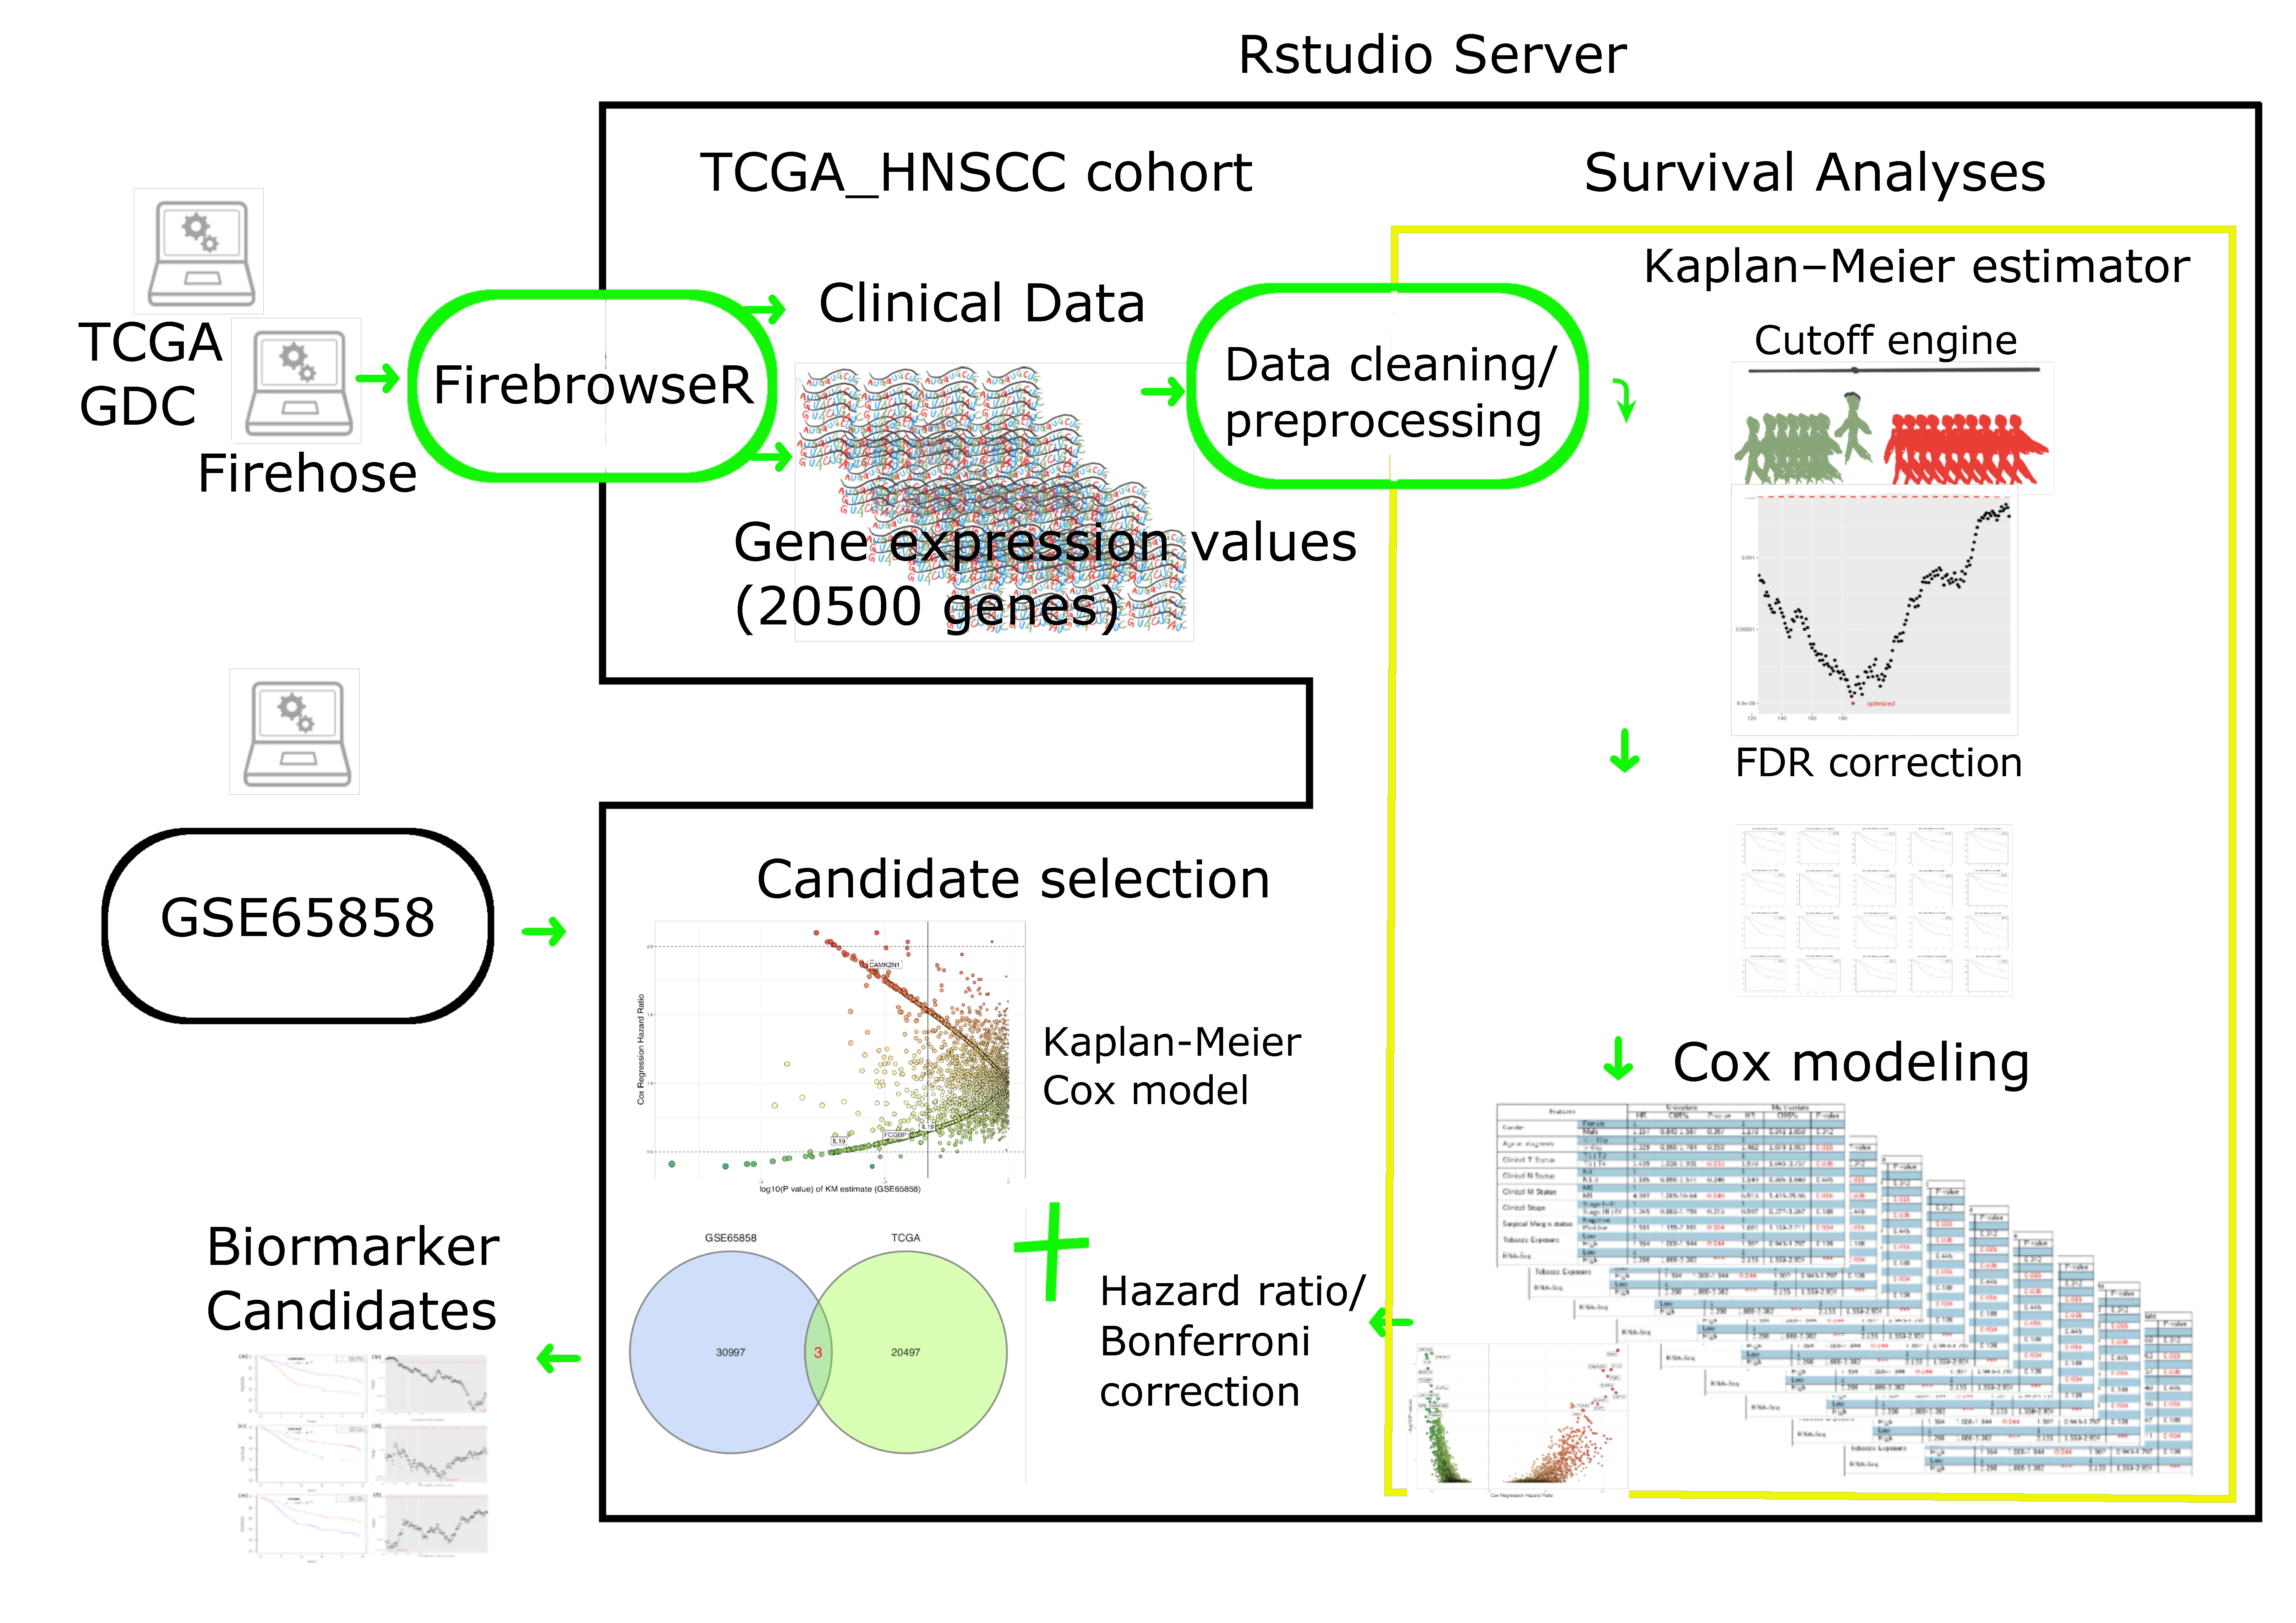
\includegraphics[width =\textwidth, height = 0.6\textheight, keepaspectratio]{Figure_1_manuscript_workflow} % .PDF is better than .png
%, height=8cm
%\caption % , step 1 (\textcolor{blue}{blue line}: main procedure) and step 2 (\textcolor{orange}{orange line}: analysis export).
%Step 3 (purple line: dealing with surgical margin).
\bcaption{A workflow of \acrshort{hnscc} biomarker discovery.}
{The workflow includes data retrieval from the TCGA GDC data portal, data processing with merging and cleaning, and then performing the survival analyses (within \textcolor{yellow}{yellow} square). The Cutoff engine (in R script: cutofFinder\_func.HNSCC.R, a serial cutoff for grouping patients with \textcolor{asparagus}{low} or \textcolor{red}{high} expression of a specific gene, to yield a collection of \protect\textit{P} values; please see Materials and Methods section for details) might calculate all possible Kaplan--Meier \protect\textit{P} values (corrected by \acrlong{fdr}, FDR, method) to find the optimal cutoff value of gene expression for subsequent Cox modeling.
The candidate selection performs (1) dissecting and selection of candidate genes with further Bonferroni adjusted \protect\textit{P} values and the hazard ratios of a Cox model, based on the results from the survival analyses;
(2) survival analyses of the other HNSCC dataset (GSE65858) using Kaplan--Meier estimates (with FDR corrections) and Cox modeling.\\
The biomarker candidates were consensus results of TCGA and GSE65858. 
(HNSCC: head and neck squamous cell carcinoma; TCGA: the Cancer Genome Atlas; RNA-Seq: RNA sequencing; GDC: Genomic Data Commons.)}
% Description:1) FDR correction of Kaplan--Meier \protect\textit{P} values during Cutoff finding; and 2) Bonferroni correction of Kaplan--Meier \protect\textit{P} values after Cox modeling for candidate selection.

\end{minipage}
%\end{figure}

\clearpage

\section{Results}


\begin{outline}

\1 Aliquam blandit faucibus nisi, sit amet dapibus enim tempus eu

\2 Nulla commodo, erat quis gravida posuere
\1 elit lacus lobortis est, quis porttitor odio mauris at libero
\1 Nam cursus est eget velit posuere pellentesque
\1 Vestibulum faucibus velit a augue condimentum quis convallis nulla gravida

\end{outline}


\clearpage

\begin{figure}[hbt!]
\centering
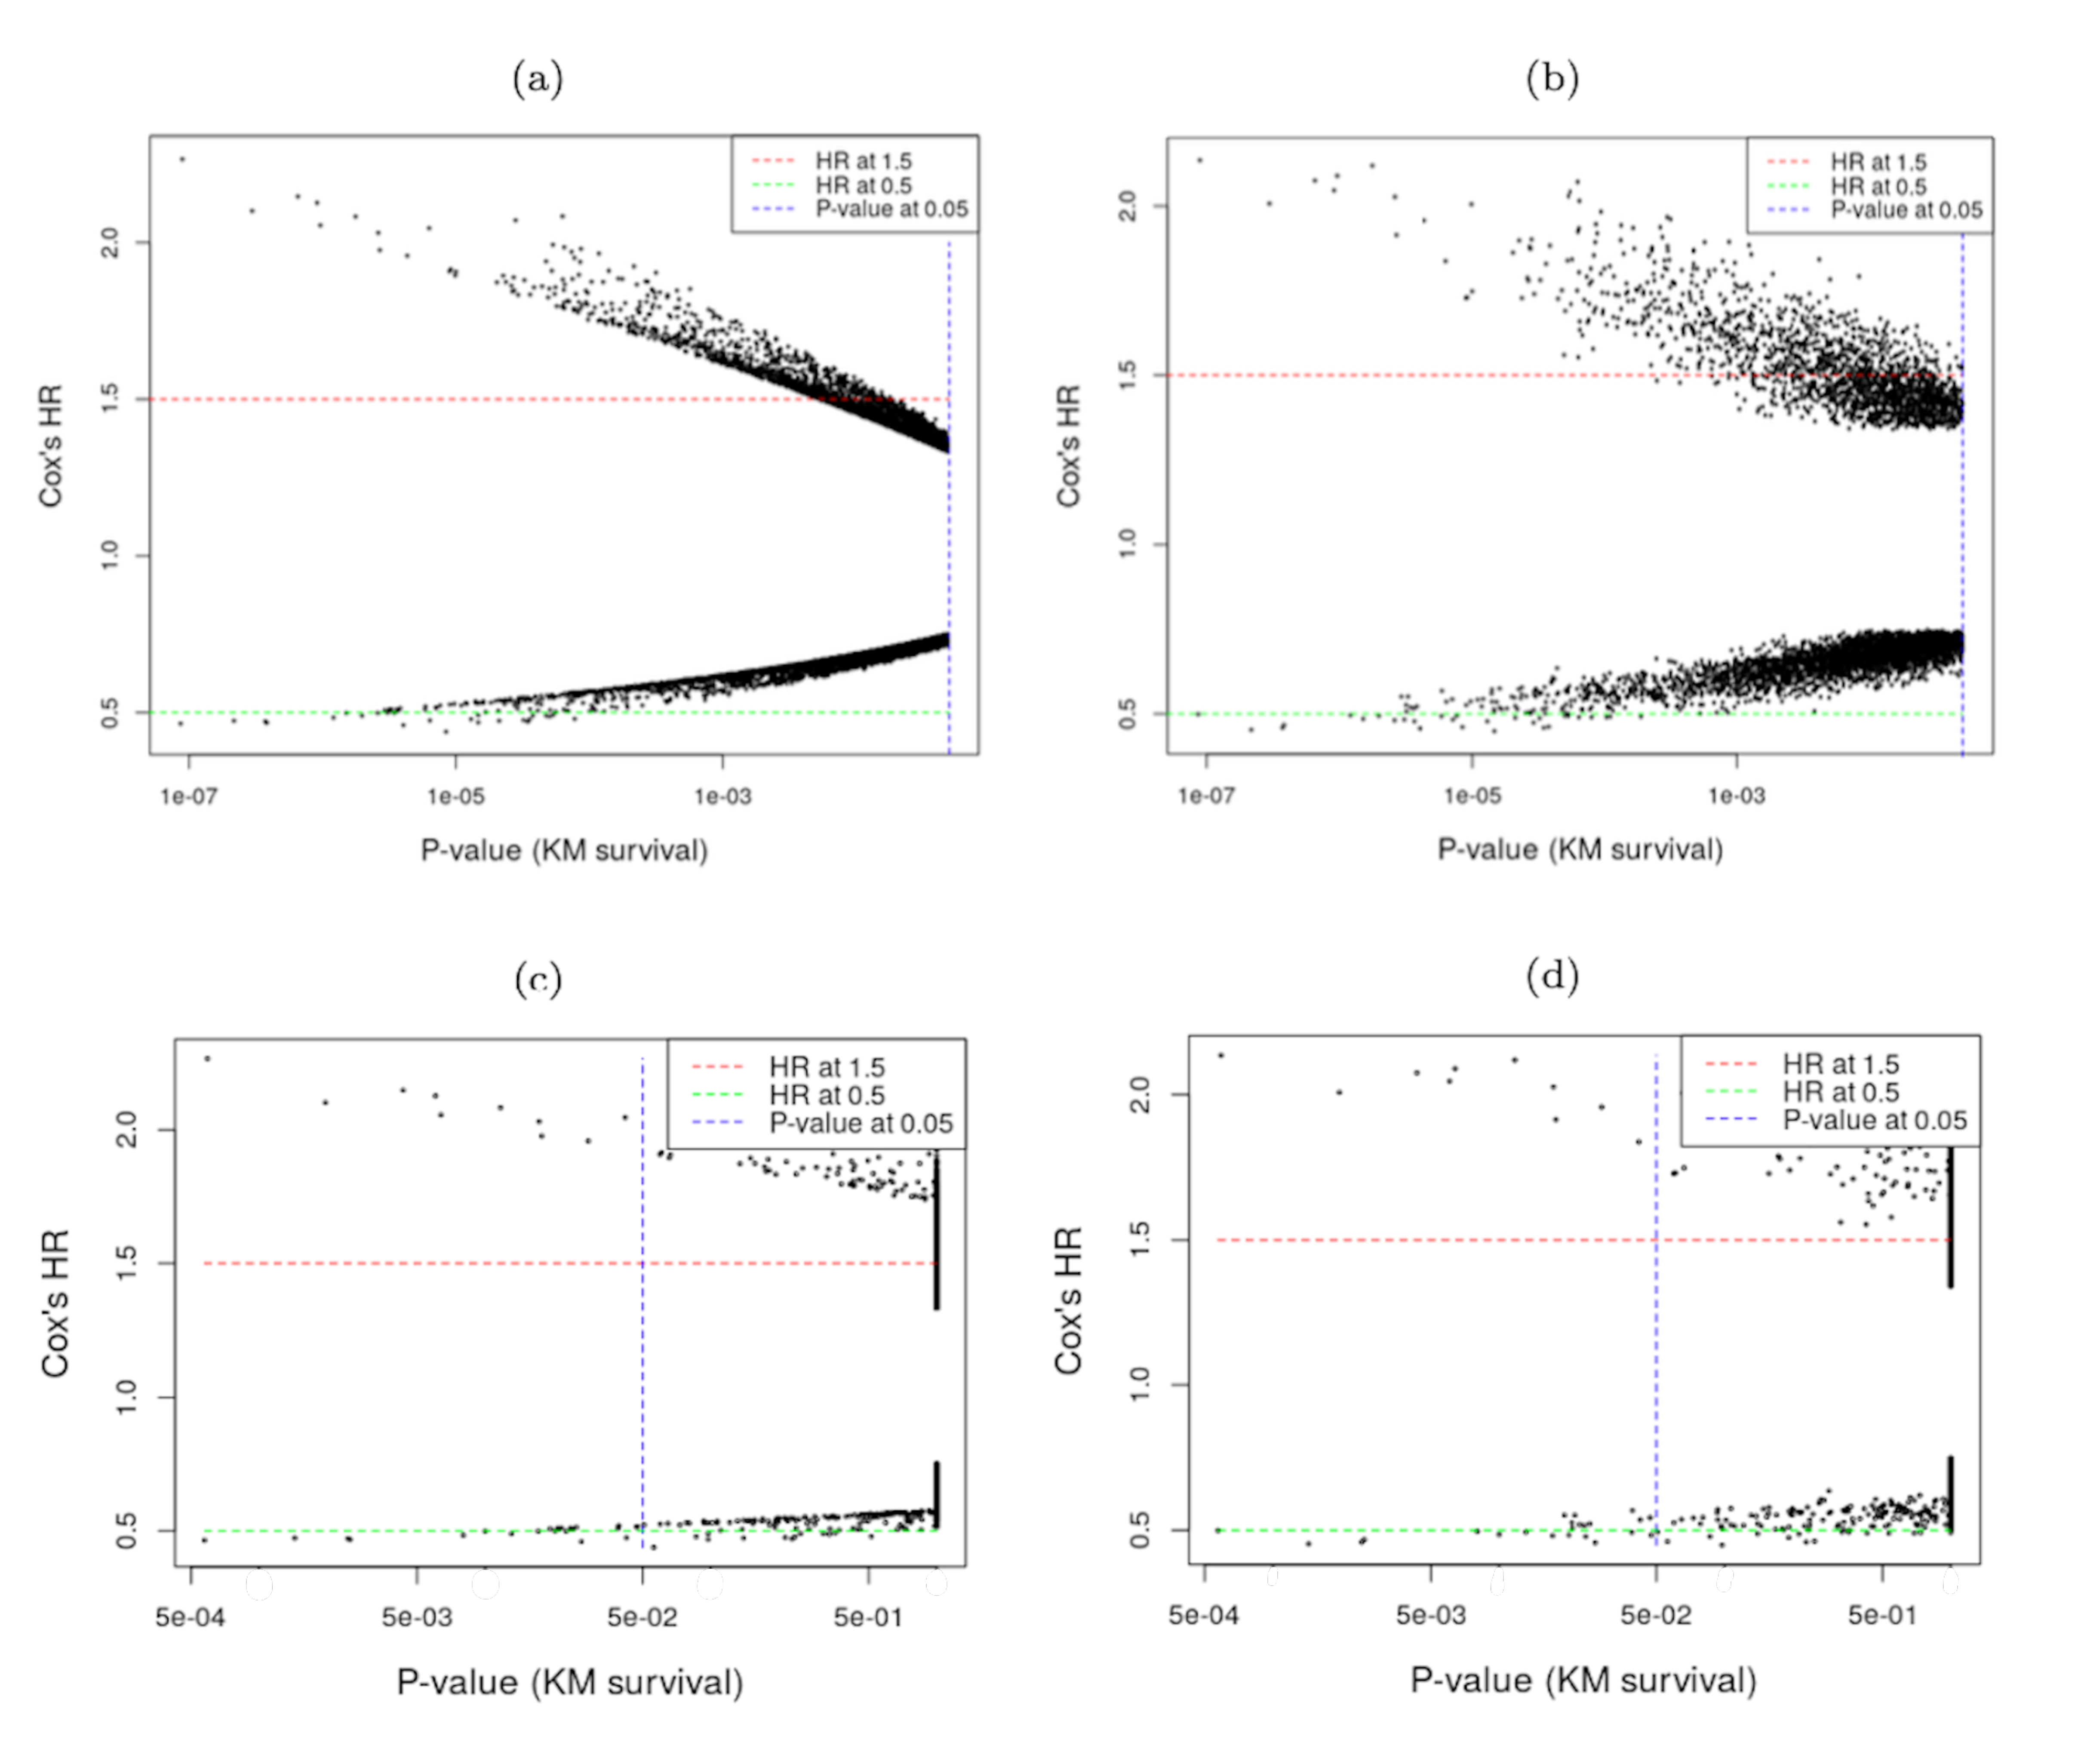
\includegraphics[width =\textwidth, height = 0.6\textheight, keepaspectratio]{Figure2.pdf}
\bcaption{The initial progress of candidate selection from the TCGA \acrshort{hnscc} cohort.}{The \protect\textit{P} value of Kaplan--Meier survival was one of the selection criteria.
The effect size was estimated by Cox's hazard ratio.
Initial trial step: (a) univariate HR versus FDR-adjusted \protect\textit{P} value; (b) multivariate HR versus FDR-adjusted \protect\textit{P} value.
After stringent restriction by Bonferroni-adjusted \protect\textit{P} values and Cox's HR, a few top-ranked genes are shown by
(c) univariate HR versus Bonferroni-adjusted \protect\textit{P} value;  (d) multivariate HR versus Bonferroni-adjusted \protect\textit{P} value.
(TCGA: \acrlong{tcga}; HR: hazard ratio; FDR: \acrlong{fdr})}
\end{figure}

\clearpage

\begin{figure}[hbt!]

% TCGA FDR Pvalue of CAMK2N1 (1.628308e-05), IL19 ( 6.543871e-06), FCGBP (4.827833e-05), CALML5 (0.0001970348)
\setlength{\unitlength}{1cm}
\begin{picture}(15, 20) %(1,0.55038404)%
\centering
  \put(0,0){\includegraphics[width=14cm]{Figure_4_CAMK2N1_CALML5_FCGBP.pdf}}%
  \put(2.5, 14.3){\fontfamily{qcr}\selectfont
  \tiny *\protect\textit{P} = \num{1.63e-05}}%CAMK2N1
    \put(2.5, 9.45){\fontfamily{qcr}\selectfont
  \tiny *\protect\textit{P} = \num{1.97e-4}}%IL19 6.54e-06 -> CALML5 0.0001970348
    \put(2.5, 4.55){\fontfamily{qcr}\selectfont
  \tiny *\protect\textit{P} = \num{4.83e-05}}%FCGBP

%\begin{annotationimage}{width=15cm}{Figure_4_CAMK2N1_IL19_FCGBP.pdf}
%\includegraphics[width=15cm]{Figure_4_CAMK2N1_IL19.pdf}
%\draw[annotation left = {Aries at 0.3}]

%\end{annotationimage}
\end{picture}%

\bcaption{Kaplan--Meier survival analyses, by cutoff finding.}
{The Kaplan--Meier curves of (a) CAMK2N1, (c) CALML5, and (e) FCGBP with optimal \protect\textit{P} values. 
((b) the cutoffs derived from it's cumulative \protect\textit{P} value plot).
%(c) Kaplan--Meier plot of IL19 under optimal \protect\textit{P} value;
((d) the cutoffs derived from it's cumulative \protect\textit{P} value plot).
(e) Kaplan--Meier plot of FCGBP under optimal \protect\textit{P} value.\\
%The optimal cutoff value for CAMK2N1 is 
The cutoffs in the cumulative \protect\textit{P} value plots of (b) CAMK2N1, (d) CALML5, and (f) FCGBP, respectively,
show that over 50\% of those unadjusted \protect\textit{P} values derived by the sliding-window cutoff-finding procedure are below 0.001.\\
(* \protect\textit{P}: \protect\textit{P} value adjusted by \acrlong{fdr}, \acrshort{fdr})
}
\end{figure}

\clearpage

\section{Discussion}
\subsection{The Three Biomarkers in Cancer}

\begin{outline}

\1 Aliquam blandit faucibus nisi, sit amet dapibus enim tempus eu

\2 Nulla commodo, erat quis gravida posuere
\1 elit lacus lobortis est, quis porttitor odio mauris at libero
\1 Nam cursus est eget velit posuere pellentesque
\1 Vestibulum faucibus velit a augue condimentum quis convallis nulla gravida

\end{outline}


\clearpage

\subsubsection*{The Protein/Pathology Atlas} %still TCGA's RNA-Seq (ok)

\begin{outline}

\1 Aliquam blandit faucibus nisi, sit amet dapibus enim tempus eu

\2 Nulla commodo, erat quis gravida posuere
\1 elit lacus lobortis est, quis porttitor odio mauris at libero
\1 Nam cursus est eget velit posuere pellentesque
\1 Vestibulum faucibus velit a augue condimentum quis convallis nulla gravida

\end{outline}


\clearpage

\subsubsection*{Literature Review} % literature (ok)

\begin{outline}

\1 Aliquam blandit faucibus nisi, sit amet dapibus enim tempus eu

\2 Nulla commodo, erat quis gravida posuere
\1 elit lacus lobortis est, quis porttitor odio mauris at libero
\1 Nam cursus est eget velit posuere pellentesque
\1 Vestibulum faucibus velit a augue condimentum quis convallis nulla gravida

\end{outline}


\clearpage

\subsection{Feature Selection for Survival Modeling} % Even there are many $X_1 ... X_n$ physical and social features of patients available for survival modelling in the TCGA.

\begin{outline}

\1 Aliquam blandit faucibus nisi, sit amet dapibus enim tempus eu

\2 Nulla commodo, erat quis gravida posuere
\1 elit lacus lobortis est, quis porttitor odio mauris at libero
\1 Nam cursus est eget velit posuere pellentesque
\1 Vestibulum faucibus velit a augue condimentum quis convallis nulla gravida

\end{outline}


\clearpage

\subsection{The Purpose of Sliding-window Cutoff Selection}

\begin{outline}

\1 Aliquam blandit faucibus nisi, sit amet dapibus enim tempus eu

\2 Nulla commodo, erat quis gravida posuere
\1 elit lacus lobortis est, quis porttitor odio mauris at libero
\1 Nam cursus est eget velit posuere pellentesque
\1 Vestibulum faucibus velit a augue condimentum quis convallis nulla gravida

\end{outline}


\clearpage

\subsection{Technical Considerations}

\begin{outline}

\1 Aliquam blandit faucibus nisi, sit amet dapibus enim tempus eu

\2 Nulla commodo, erat quis gravida posuere
\1 elit lacus lobortis est, quis porttitor odio mauris at libero
\1 Nam cursus est eget velit posuere pellentesque
\1 Vestibulum faucibus velit a augue condimentum quis convallis nulla gravida

\end{outline}


\clearpage

\subsection{Limitations of the Study}


\begin{outline}

\1 Aliquam blandit faucibus nisi, sit amet dapibus enim tempus eu

\2 Nulla commodo, erat quis gravida posuere
\1 elit lacus lobortis est, quis porttitor odio mauris at libero
\1 Nam cursus est eget velit posuere pellentesque
\1 Vestibulum faucibus velit a augue condimentum quis convallis nulla gravida

\end{outline}


\clearpage

\subsection{Future Directions in Translational Medicine}

\begin{outline}

\1 Aliquam blandit faucibus nisi, sit amet dapibus enim tempus eu

\2 Nulla commodo, erat quis gravida posuere
\1 elit lacus lobortis est, quis porttitor odio mauris at libero
\1 Nam cursus est eget velit posuere pellentesque
\1 Vestibulum faucibus velit a augue condimentum quis convallis nulla gravida

\end{outline}


\clearpage

\subsubsection{Proteomics Validation}

\begin{outline}

\1 Aliquam blandit faucibus nisi, sit amet dapibus enim tempus eu

\2 Nulla commodo, erat quis gravida posuere
\1 elit lacus lobortis est, quis porttitor odio mauris at libero
\1 Nam cursus est eget velit posuere pellentesque
\1 Vestibulum faucibus velit a augue condimentum quis convallis nulla gravida

\end{outline}


\clearpage

\subsubsection{Laboratory Validation}

\begin{outline}

\1 Aliquam blandit faucibus nisi, sit amet dapibus enim tempus eu

\2 Nulla commodo, erat quis gravida posuere
\1 elit lacus lobortis est, quis porttitor odio mauris at libero
\1 Nam cursus est eget velit posuere pellentesque
\1 Vestibulum faucibus velit a augue condimentum quis convallis nulla gravida

\end{outline}


\clearpage

\subsubsection{Cancer Type-agnostic Study}

\begin{outline}

\1 Aliquam blandit faucibus nisi, sit amet dapibus enim tempus eu

\2 Nulla commodo, erat quis gravida posuere
\1 elit lacus lobortis est, quis porttitor odio mauris at libero
\1 Nam cursus est eget velit posuere pellentesque
\1 Vestibulum faucibus velit a augue condimentum quis convallis nulla gravida

\end{outline}


\clearpage

\subsubsection{Holistic Cancer Care} 


\begin{outline}

\1 Aliquam blandit faucibus nisi, sit amet dapibus enim tempus eu

\2 Nulla commodo, erat quis gravida posuere
\1 elit lacus lobortis est, quis porttitor odio mauris at libero
\1 Nam cursus est eget velit posuere pellentesque
\1 Vestibulum faucibus velit a augue condimentum quis convallis nulla gravida

\end{outline}


\clearpage


\begin{figure}[hbt!]
\centering
\includegraphics[width =\textwidth, height = 0.6\textheight, keepaspectratio]{Figure_5_holisticCare.pdf}
\bcaption{The concept of holistic care for \acrshort{hnscc} patients.}
{\\Beyond carcinogenesis: In the mind--brain--body axis, a stressful environment (giant \textcolor{black}{black} arrow) will trigger an emotional response. The subconscious mind (brain) will release stress hormones and inflammation signals in response to the emotion. The physical body's internal environment (cells) alters epigenetic control in gene regulation and mRNA expression. Over a long incubation time, the tissue/cells will be transformed into dysplasia and then malignancy (e.g., HNSCC) with help from known carcinogens.\\
Cancer care: Holistic care should take care of cancer patients' spiritual, emotional, physical, and socioeconomic needs. Physical care will be carried out by medication therapy or surgery. After establishing a therapeutic relationship (TR), the physicians' spiritual properties (empathy, sympathy, and compassion) will engage their patients and recover their self-compassion to gain resilience against the disease through their mind--brain--body axis.
Thus, we suggest that electric healthcare records (EHR) should include physical, pathological, and psychological data, and even more spiritual information. The \acrshort{tcga} might collect those "holistic features"  (\textcolor{green}{green} dashed line) for further study of personalized medicine.}
\end{figure}

\clearpage

\section{Materials and Methods} % 4
\subsection{Patient Cohort} 
\subsubsection{RNA Sequencing Data} 

\begin{outline}

\1 Aliquam blandit faucibus nisi, sit amet dapibus enim tempus eu

\2 Nulla commodo, erat quis gravida posuere
\1 elit lacus lobortis est, quis porttitor odio mauris at libero
\1 Nam cursus est eget velit posuere pellentesque
\1 Vestibulum faucibus velit a augue condimentum quis convallis nulla gravida

\end{outline}


\clearpage

\subsubsection{Clinical Data} 

\begin{outline}

\1 Aliquam blandit faucibus nisi, sit amet dapibus enim tempus eu

\2 Nulla commodo, erat quis gravida posuere
\1 elit lacus lobortis est, quis porttitor odio mauris at libero
\1 Nam cursus est eget velit posuere pellentesque
\1 Vestibulum faucibus velit a augue condimentum quis convallis nulla gravida

\end{outline}


\clearpage

\subsection{Cutoff Finder Core Engine}

\begin{outline}

\1 Aliquam blandit faucibus nisi, sit amet dapibus enim tempus eu

\2 Nulla commodo, erat quis gravida posuere
\1 elit lacus lobortis est, quis porttitor odio mauris at libero
\1 Nam cursus est eget velit posuere pellentesque
\1 Vestibulum faucibus velit a augue condimentum quis convallis nulla gravida

\end{outline}


\clearpage

\subsection{Statistical Consideration for Survival Analysis}

\begin{outline}

\1 Aliquam blandit faucibus nisi, sit amet dapibus enim tempus eu

\2 Nulla commodo, erat quis gravida posuere
\1 elit lacus lobortis est, quis porttitor odio mauris at libero
\1 Nam cursus est eget velit posuere pellentesque
\1 Vestibulum faucibus velit a augue condimentum quis convallis nulla gravida

\end{outline}


\clearpage

\subsection{Biomarker Selection and Validation}


\begin{outline}

\1 Aliquam blandit faucibus nisi, sit amet dapibus enim tempus eu

\2 Nulla commodo, erat quis gravida posuere
\1 elit lacus lobortis est, quis porttitor odio mauris at libero
\1 Nam cursus est eget velit posuere pellentesque
\1 Vestibulum faucibus velit a augue condimentum quis convallis nulla gravida

\end{outline}


\clearpage


\section*{Conclusions} % 5


\begin{outline}

\1 Aliquam blandit faucibus nisi, sit amet dapibus enim tempus eu

\2 Nulla commodo, erat quis gravida posuere
\1 elit lacus lobortis est, quis porttitor odio mauris at libero
\1 Nam cursus est eget velit posuere pellentesque
\1 Vestibulum faucibus velit a augue condimentum quis convallis nulla gravida

\end{outline}


\clearpage

%------------------------------------------------

\section*{Citations}

An example of the \texttt{\textbackslash cite} command to cite within the presentation:

This statement requires citation \cite{Smith:2012qr}.

\clearpage

%------------------------------------------------
\subsection*{Užití}

\textit{Informační systém nákup letenek} bude použit v interakci se třemi skupinami uživatelů - Administrátor, Zaměstnanec a zákazník. 

\begin{multicols}{3} % Divide text into multiple columns
\mygreen{Sed diam enim, sagittis nec} condimentum sit amet, ullamcorper sit amet libero. \mybrown{Aliquam vel dui orci}, a porta odio. \myred{Nullam id suscipit} ipsum. \myblue{Aenean lobortis} commodo sem, ut commodo leo gravida vitae. Pellentesque vehicula ante iaculis arcu pretium rutrum eget sit amet purus. Integer ornare nulla quis neque ultrices lobortis. Vestibulum ultrices tincidunt libero, quis commodo erat ullamcorper id.
\end{multicols}

\clearpage
%%%%%%%
\thispagestyle{empty} % No slide header and footer

\bibliographystyle{unsrt}
\bibliography{sample}

\clearpage

%------------------------------------------------

\thispagestyle{empty} % No slide header and footer

\begin{tikzpicture}[remember picture,overlay] % Background box
\node [xshift=\paperwidth/2,yshift=\paperheight/2] at (current page.south west)[rectangle,fill,inner sep=0pt,minimum width=\paperwidth,minimum height=\paperheight/3,top color=mygreen,bottom color=mygreen]{}; % Change the height of the box, its colors and position on the page here
\end{tikzpicture}
% Text within the box
\begin{flushright}
\vspace{0.6cm}
\color{white}\sffamily
{\bfseries\LARGE Comments and Suggestions\par} % Request for questions text
\vfill
\end{flushright}

%----------------------------------------------------------------------------------------

\end{document}